In order to evoke flow state in the player, the game must be designed in such a way that the task and its environment enhance immersion and engagement. As rhythm games differ from other game genres that include narratives, plot, quests and objectives, it may seem that flow state applicates differently in this genre. However, the core elements of flow state are objectively the same as in any other game or activity.
Firslty, it is crucial to understand the fundamentals of flow state and its importance in the context of video games. As Jenova Chen describes in his MFA thesis, Mihaly Csikszentmihaly distinguishes eight component that are required to achieve the flow state:
\begin{quote}
According to Mihaly Csikszentmihalyi's well-documented research and wide-scale
gathering of personal observations, the phenomenology of Flow has eight major
components.
\begin {itemize}
\item A challenge activity that requires skills
\item The merging of action and awareness
\item Clear goals
\item Direct feedback
\item Concentration on the task at hand
\item The sense of control
\item The loss of self-consciousness
\item The transformation of time
\end {itemize}
Not all of these components are needed for flow to be experienced. [Csikszentmihalyi 1990](Chen 2006: 7).
\end{quote}

These components are crucial to evoke flow state throughout various activities, including video games. Regarding games, there are three core elements that Jenova Chen indentifies: 
\begin {itemize}
\item As a premise, the game is intrinsically rewarding, and the player is up to play the game.
\item The game offers right amount of challenges to match with the player's ability, which allows him/her to delve deeply into the game.
\item The player needs to feel a sense of personal control over the game activity. 
\end {itemize}
As a result, the game will make player lose track of time and self-consciousness. (Chen 2006: 7)

Regarding rhythm games, such criteria are meet through merging the game's mechanics with music. As mentioned in the curator's note of “A MAZE. Interact” \cite{MAZE} catalogue: "Music games exemplify the generally ambivalent nature of rules: whilst restricting action space, they produce new opportunities for interacting with music.” (Liebe/Wiedemann 2010: 5). Performing the task is rewarding in itself, as the player can feel the satisfation of hitting the notes to the rhythm of the music instantly, no matter the difficulty. As the player becomes more skilled at the game, they can unlock and play more difficult levels, always adjusting the game's difficulty to their current skill level. Following the definition of flow state, the balance between skill and challenge plays fundamental role in maintaining the flow state. If the task difficulty is too high, the player is unable to enter flow state, as the task is evoking anxiety. On the other hand, if the capabilities of the player exceed the challenge, the player will become bored. The safe space between anxiety and boredom is determined as \textit{flow zone}.

\begin{figure}[h]
    \centering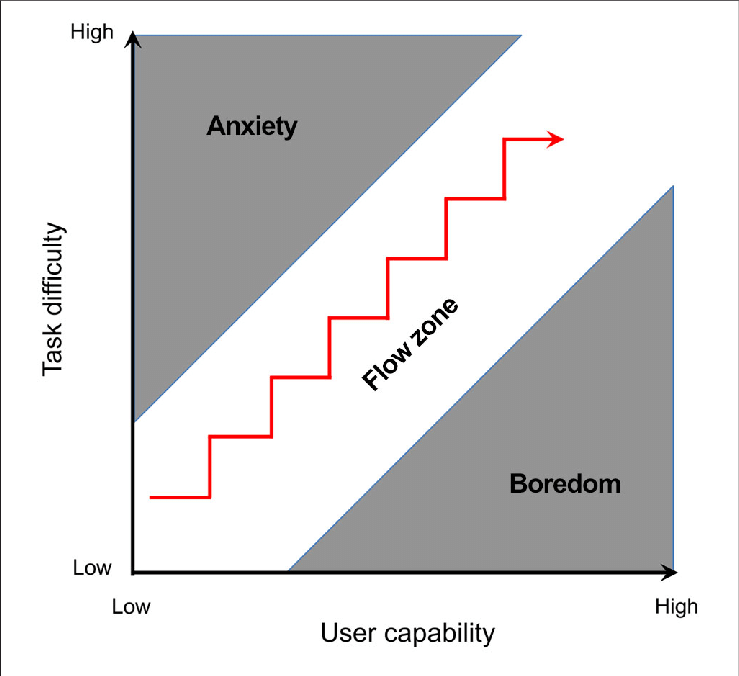
\includegraphics[scale=0.3]{obrazki/flowstategraph.png}
    \caption{\textit{Csikszentmihalyi's flow state} -- graph showing how does the balance between the player's skill and the game's challenge influence the flow state.
    \cite{csikszentmihalyi1990flow}}
    \label{fig:flowstategraph}
\end{figure}

In rhythm games, as the player can always pick the desired difficulty level, it is easy for the player to maintain the flow state. If there is a difficulty that was too hard in the past, the player can always come back to it later, when they feel more confident with their capabilities. This replayability also allows the player to improve their previous scores, which can be a source of motivation to keep playing the game. Consequently, rhythm games meet the critera for both casual and hardcore gaming, as Jesper Juul describes in his book: \textit{A Casual Revolution: Reinventing Video Games and Their Players}\cite{casualrevolution}:
\begin{quote}
    In other words, these games are very different depending on what players are trying to achieve. For players who want to relax playing a song they like, the games fulfill the role of casual games where even an imperfect performance of a song on an easy level of difficulty can be a satisfying experience. However, for players who want to master the games or win a competition, the games' punishment structures match traditional hardcore design. In this case, the player must keep replaying a given song in order to perfect his or her skills (Juul 2010: 129).
\end{quote}

Beside maintaining the flow state, games must also be entertaining during the flow zone. As rhythm games revolve around music, it can be naturally achieved through the inclusion of music, which in itself is a source of entertainment. As usual, music is constructed in such a way that it catches the attention of the listener through its structure. The six primary parts of the song can correspond to the gameplay. As the song starts with intro, which is usually slower, the player can familiarize with the rhythm and warm-up. As the song progresses and becomes more energetic, the player can expect more intense parts, that can be reflected in the gameplay. Such build-up prepares the player for the climax of the song, which is usually the most difficult part to play during a selected level. Typically, songs have slower parts between the intense chours, in which the player can relax and prepare for the next intense part. After another intense part, the song usually ends with a slower outro, in which the player can relax with less difficult patterns of notes. As such structure is repeated in most songs, no matter the genre, even the most novice players can quickly understand that their play will resemble the structure of music that they listen to. This feeling of familiarity can reduce the potential anxiety when trying new difficulties, therefore enhance the entertainment coming from the play. This practice may resemble a process of learning an instrument, as mentioned in \textit{A Casual Revolution: Reinventing Video Games and Their Players}\cite{casualrevolution}:
\begin{quote}
    On some level it is true that these are not real instruments, but what makes them not real? The basic experience of playing these games is that if you do not press the buttons correctly there is no music, but if you press the buttons correctly, music appears—it feels as if you are making music. Interestingly, this is quite similar to learning to play an instrument (...) (Juul 2010: 115).
\end{quote}
Because of this natural familiarity, creating a songlist that is fun to play could be more intuitive than it may seem. As Fares Kayali describes in \textit{Playing music : design, theory, and practice of music-based games} \cite{faresplayingmusic}: 
\begin{quote}
    "Since music is not completely graspable by a specific methodology, the process of formalizing music for music-based game design also depends upon its more abstract attributes. Kungel’s (2004) distinct audio parameters for movies includes dynamics, harmony, sound, melody, pause, rhythm, beat, and tempo. It provides game designers a list of parameters that can be accessed through player interaction or be changed as feedback to players." (Fares 2008: 60).
\end{quote}
With this insight in mind, game designers can choose songs for their game basing their choices on what they believe will resonate with the target audience. The music must match the game's mechanics and control device, which in most cases will fit a wide range of music genres. Knowing that music is entertaining to listen to on its own, its ability to enhance the player's experience and support a flow state is primarily dependent on how well the level design is integrated with the featured music. The audio parameters described by Kungel's should serve as a guide for game designers and as a reference for the level design and note patterns included in the song charts.

\section{Components of Flow in rhythm games}
Coming to the aspects of clear goals, the objective of playing a rhythm game can initially seem as simply playing the song. However, games without the imposed narrative are giving the player more freedom to set their own goals. As mentioned before, the player may choose if they want to play casually or hardcore. Since there are plenty of various rhythm games, players can also choose which game appeal to them the most. As highlighted by Juul: "Games without goals or with optional goals are more \textit{flexible}: they accommodate more playing styles and player types, in effect letting you choose what kind of game you want to play" (Juul, 2010: 138). This flexibility enables the player to naturally estabilish personal objectives. Liberating the player from the pressure of meeting the imposed goals makes more space for the player to actually enjoy the game and polish their skills at the same time. On the other hand, some rhythm games offer storymodes or quests that unlock new songs or levels after completion. While this may motivate the majority of players to keep playing, it also may be frustrating for those who want to have the freedom of choice right away.
As described, the approach to progression in rhythm games varies widely - from completely lacking the storymode or structured campaign, through incomporating optional mission-based elements, to featuring full storylines that must be completed in order to unlock the full content imposed by the game developers. Taking these three levels as an example, this variety of imposed objectives and progression path can be observed across different rhythm games.
Games like \textit{osu!} or \textit{StepMania} do not have any story mode or campaign, as their content is centered around the content created by the community and online leaderboards. These games lack the predefined progression system, as all of the content is available through downloading the content created by the community. Apart from being a player, users can also become creators of the content, as they can create own levels, skins or even songs. One interesting example of a collaboration between game developers and music creators is \textit{osu!}, since the game allowed to create and upload \textit{beatmaps} for any .mp3 file chosen by the \textit{beatmapper} (the user which creates the map for this particilar game). This aspect was highlighted by Fares Kayali in Playing music : design, theory, and practice of music-based games \cite{faresplayingmusic}: "Through increasing possibilities for downloadable content, music-based games also act as distribution platforms for music." (Kayali, 2008: 53). This solution raised questions about licensing music, as the original musicians were not asked if they want their songs to be used in the game - noteworthy, the game is constructed in such a way that the .mp3 file with the full song is included in the beatmap folder. For this reason, some beatmaps were removed by musicians who found out about it and were not quite happy about it (for example: Skrillex). Under pressure from allegations of using unlicensed music in the game and generating profit from it, the developer of \textit{osu!} - peppy - began to collaborate with musicians through the "featured artists" program, officially licensing songs from artists that were interested in being featured. However, beatmappers are still allowed to use any .mp3 file from their computer, so making the risk of distributing pirated music is not completely eliminated. Nevertheless, this solution created unlimited opportunities for players and content creators to gamify of any music possible, at the same time promoting musicians, as many players can be introduced to their music throughout the game. This solution has its benefits and drawbacks, but leaving aside the moral part, this level of freedom in creative work has an impact on player and community engagement. It completely replaces the narrative aspect of the game, directing the player's attention to content created by the community and the competition with other players. The game's content is created in such a way that there's always something new to play, encouraging the players to compete for the best scores on newest songs. Especially during the official and community tournaments, players are always competing on the same beatmaps. A notable element of this is the fact that beside creating the composition and shape of the level, the \textit{beatmappers} are also responsible for choosing the background image and the visual effects (storyboards) of their map. Additionally, they may include custom hitsounds that further enhance the desired experience of playing their content. As the one can observe, the example of \textit{osu!} shows that the engagement of the playerbase may not depend on the content created by the developers or the procedurality of storymodes. In this regard, the designed mechanics of the developers can simply serve as an instrument for the game community to create immersive content that evokes flow state. As players can create their own beatmaps with the music of their choice, the invocation of the flow state can be taken to the next level. For example, if a player notices that an old beatmap is poorly designed and missing important aspects, they can create their own version with adjustments. An important aspect of curating beatmaps for osu is that the beatmap need to under the procedure of testing and review in order to be qualified as ranked map - only then it can contribute to the personal scores of players and the global leaderboard. Since the map must be polished and meet certain requirements in order to be playable and ranked, the testers must also reassure that it will be entertaining to play - therefore, the acquisition of Flow Zone during playing the beatmap will be assured by the curators and community feedback. 

On the contrary, the inclusion of a lightweight mission system is present in \textit {Groove Coaster: Wai Wai Party!!!!} for Nintendo Switch. The game offers missions and challenges that require a wide range of effort and time. Some of the missions require the player to play a certain song only once, while other challenges obligate the player to play every song of a given category and difficulty level. These challenges are devoid of any narrative, which in this case is rather a better solution, take less time and leave the player with clear and obvious goals. What may be frustrating for some players, these missions are included as a progression tree that requires completing one mission to progress into the next one. As a solution, the player obtains in-game currency throughout the play and may auto-complete desired missions by spending it. Unlike \textit{osu!}, the content of \textit {Groove Coaster: Wai Wai Party!!!!} is procedurally designed by its developers, leaving the player base fully dependent on new updates and DLCs that are available within the payment. This approach to the player experience is quite different from the aforementioned \textit{osu!}, as the game has limited catalogue of content that the player may unlock and play. Therefore, games with such approach can be fully completed by the player. This approach is more similar to other games that encourage the player to play in order to fully complete the game. Although the game is designed this way, the difficulty level and the skill needed to complete the hardest songs are so high that most players will likely never manage to fully clear all expert-level songs.

An example of a game that incorporates a developed story mode is \textit{Guitar Hero III: Legends of Rock} for home consoles and PCs. The game features a single player and Co-op Career Mode. In single player Career Mode, the game puts the player in a role of a rockband member with a goal of becoming a rockstar and growing the band to the heights of fame and popularity. It is structured as a linear series of 8 tiers, presenting a fictional venue where the player performs the gigs. Each tier contains 4 or 5 songs and requires the player to complete current set of songs - the player must complete at least 3 or 4 songs of the setlist (depending of the currectly chosen difficulty) to unlock the last part of the tier: Encore and a Boss Battle, some tiers conclude only one, while others involve both. Passing the last part results in the completion of a tier. Progressing to other tiers further increase the difficulty of the songs. While passing through the songs, the player earns the in-game currency, which the player may spend in Shop in order to unlock new guitars, heroes and bonus songs. The Co-op career mode is similar to the singleplayer mode, but it features different setlist (songs) and lacks the unique Boss Battles. As observed, the Career Mode consists `of three main, defined objectives: complete set numer of songs, defeat a boss or play an encore, progress to the next tier. Such structure provide clear goals for the player, thereby making the player immersed in the task at hand. The sequence of short-term missions helps the player to maintaing focus and lead to long-term mastery, as the player is constantly improving their skills throughout the play. As the Career Mode starts with simpler songs and gradually introduce faster tempo and more complex patterns of notes, the aspect of increasing challenge ensures that the player will be enclosed in the Flow Zone, between the anxiety and boredom. Although the campaign is linear, the player has the ability to choose song order within setlist, providing the sense of control over the course. On top of that, the Career Mode includes elements that enhance the player's immersion - it portrays the player's progression as an adventure of a rockband, which is additionally presented through the cartoon-like animated cutscenes and the visual design of the game. The game's UI, artstyle and visuals further complement the experience of feeling like a member of a rockband, as the whole theme of the game revolves around rock music and the lifestyle of a rockstar. Obviously, as previously described in Chapter 2, the inclusion of real-life rock music which is present in every Guitar Hero game, is a significant aspect of evoking the flow state - in this case, the setlist of Career Mode also includes rock music created by real-life musicians. As Kayali Fares writes in \textit{Playing music : design, theory, and practice of music-based games} \cite{faresplayingmusic}: "With Guitar Hero, Harmonix has successfully revived the vibe of rock’ n’ roll" (Kayali 2008: 66).

The element of time transformation and the loss of self-consciousness are especially emphasized in arcade rhythm games. For practical reasons, arcade parks are often located in dark spaces, making the screens of arcade machines more visible. They are also tightly packed with machines, as renting more space can be costly. This dense arrangement of loud, flashy machines enhances the sensory-rich atmosphere. The unique environment, focused on games and entertainment, creates the illusion of being separated from the everyday world, making it easier to lose track of time. Arcade rhythm games, with their distinctive cabinets and controllers, stand out from other types of arcade machines. One of such arcade rhythm games is \textit{maimai} game series, developed by Sega and first released in 2012. The game include both singleplayer and multiplayer mode, as its arcade machine consists of 2 player slots. The main display is a large circular touchscreen, surrounded by 8 buttons that are spaced evenly on the edges of the screen. In \textit{maimai}, the core gameplay revolves around responding to ring notes, which emerge from the center of the screen and travel outward toward the edge of the screen, aligning with one of the eight physical buttons arranged around the perimeter (judgement line). These are large, responsive pads that light up and provide tactile feedback, integral to the gameplay. Additionally, tap notes and slider notes appear on the touchscreen itself, requiring the player to tap or swipe on the screen with their hand. Similarly to other rhythm games, the player's input produces in-game hit sounds and visual effects, creating a satisfying feedback loop that enhances immersion and flow state. As the game's cab include two player slots, it encourages to socialize with other players. The players can decide if they want to compete with each other in VS mode, or play along in Sync Mode - in which the objective is pursue the best score possible and synchronization, measured as a percentage. The game cab includes an IC card reader, on which the players can saves their scores, unlock additional content and customize their personal profiles with currency obtained through achievements and events that include time-limited missions. Player profiles show not only best singleplayer scores, but also include Max Sync, which shows the highest combo (consecutive hit of notes without missing) achieved with the other player in Sync Mode. Including such mechanics and in-game content that revolves around socializing with other players, the game encourages the players to play together and share their experience. Even while waiting in the queue for play, the players can talk to each other and watch the other players and cheer for them, which creates a sense of community. Combining this with the setting of arcade parks, the players can easily lose track of time and become fully immersed in the game and it's environment. Taking into account the social aspect, the transformation of perceived time is further enhanced. This meaning of socializing during the play is described by Jesper Juul in \textit{A Casual Revolution: Reinventing Video Games and Their Players} \cite{casualrevolution}:

\begin{quote}
    Our pursuit of game goals makes the playing of games emotional even if we cannot point to any emotional content in the rules of a specific game. I think this can be
    extended to multiplayer games by thinking about how goals work in social contexts: players play for personal goals, are aware of the goals of other players, and the shared understanding of intentionality makes game actions socially meaningful (Juul 2008: 126).
\end{quote}

This aspect of socializing and sharing the experience with other players is crucial in evoking flow state, as it creates a sense of community and belonging. The players are not only focused on their own performance, but also on the performance of their friends or other players, which can enhance the overall experience. This aspect is especially important in arcade rhythm games, where the environment and the social aspect play a significant role in creating an immersive experience that evokes flow state.
